\documentclass[sigconf,12pt]{acmart}
\usepackage{setspace}
\usepackage{booktabs} % For formal tables
\usepackage{times}
\usepackage{wrapfig}
\usepackage[outdir=./]{epstopdf}
% Copyright
\setcopyright{none}

%Conference
\acmConference[6UAR'17]{MIT 6.UAR}{MAY 2017}{
  Cambridge, Massachusetts} 

%%%%%%%%%%%%%%%%%%%%%%%%%%%%%%%%%%%%%%%%%%%%%

%%%%%%%%%%%%  Your Edits Below  %%%%%%%%%%%%

%%%%%%%%%%%%%%%%%%%%%%%%%%%%%%%%%%%%%%%%%%%%%

\begin{document}
\title{Localization of the Heart in MRI Scans}

\author{Courtney Guo}
\affiliation{%
  \institution{Massachusetts Institute of Technology}
}
\email{ckguo@mit.edu}

\author{Danielle Pace}
\affiliation{%
  \institution{Massachusetts Institute of Technology}
}
\email{dfpace@csail.mit.edu}

\author{Polina Golland}
\affiliation{%
  \institution{Massachusetts Institute of Technology}
}
\email{polina@csail.mit.edu}


\begin{abstract}
\doublespacing
Congenital heart disease (CHD) affects many children around the world, which sometimes requires extensive surgery planning. For doctors to be able to plan surgeries, it is helpful if scans of the heart are accurately labelled with the different substructures of the heart. Some work has been done to address the issue of image segmentation in hearts with CHD [1], but these methods still require some user input and therefore are not fully automatic.

In this work, we aim to develop methods to localize the heart in MRI scans of patients with congenital heart disease. We perform localization by applying a regression forest to the MRI scans of the patient, to find the bounding boxes of the structures within the heart. [STATE RESULTS HERE] %\footnote{This is an abstract footnote}
\end{abstract}


\maketitle

\begin{doublespacing}
%If you would like to sections to be split across multiple files,
%add them below in the same format as samplebody.
\section{Introduction}
Millions of children around the world are born with congenital heart defects, which may require surgery to be treated. For doctors to effectively plan surgery, it is useful if a model of the heart can be 3D-printed. This requires the scans of the patient to be segmented, which means each voxel must be labeled with what section it belongs to. Traditionally, this means that an expert must manually label each voxel in the image with whether or not it belongs in the bloodpool, myocardium, or outside the heart. Currently, patient-specific 3D heart models are underused because it takes around 4-8 hours to manually segment cardiac MRI images, since each contains 100-150 slices. There have been algorithms developed to segment the heart in normal adult patients, one of the most popular being atlas segmentation, which uses a fully segmented heart as a reference and tries to align a patient's heart to the given reference. However, atlas-based methods do not work well on children with congenital heart disease (CHD) due to the irregular location or shapes of the organs. An active learning method has been developed to segment images of hearts with CHD, but because it requires user input it is not fully automatic.

This paper proposes an alternative method to aid the segmentation of hearts with CHD. Segmenting images of hearts with CHD as opposed to healthy hearts is an additional challenge, because hearts with CHD may have incomplete or missing structures, or structures located in different areas compared to healthy hearts. Therefore, many traditional methods for segmenting these images do not work well. The method proposed in this paper attempts to address these challenges. A first step to segmentation is localizing regions of interest, which means locating bounding boxes around those regions, which will assist downstream processing.

The method proposed in this paper localizes the heart in patients with congenital heart disease, using random forests. [SUMMARIZE RESULTS]

\section{Related Work}
One method for segmentation of the heart in children with CHD is an interactive algorithm based on partial manual segmentation [1]. The user is directed to manually label 10-15 slices uniformly distributed throughout the 3D volume. The algorithm then segments each remaining slice according to its closest reference slices. To segment a patch, the algorithm finds the k most similar patches in the set of relevant reference regions, and ``similarity" depends on patch intensities, gradients, and positions, and each pixel is labeled according to a majority vote. This algorithm greatly reduces the amount of time needed to segment a heart to less than 1 hour of manual labelling and 1 hour of algorithm runtime. However, since the algorithm still requires user interaction, it is not fully automatic. The algorithm proposed in this paper is fully automatic; although it runs in [INSERT HOURS HERE]	6? hours once trained, it still saves doctors' time and allows them to devote their attention to other tasks.

Regression forests have also been shown to do well in image segmentation, specifically the detection and localization of organs. A. Criminisi has applied regression forests to learn the non-linear mapping from voxels directly to organ position and size [2]. The regression forest groups voxels with similar features or similar field of views together, and learns an estimate of the bounding boxes of each organ using the training data that reaches that node. Intuitively, each voxel contributes varying degrees of confidence to the estimates of the location and size of every organ. When applied on real datasets, the forest learns to recognize key indicators (such tips of the ribs or vertebrae) and those pixels provide high confidence estimates of where certain organs are located. Criminisi then compared these results against other methods, including Elastix and Simplex methods, as well as atlas methods, and showed that the regression forest method was superior in accuracy. This paper applies the regression forest methods used by Criminisi to children with CHD.

\section{Regression Random Forests}
This paper develops a method to localize the heart in 3D MRI scans of patients with CHD, based on regression random forests. A random forest is a supervised machine learning model that consists of many decision trees, in which the training phase of each tree contains some amount of randomness. A decision tree is a flow-chart like structure in which each node is a Boolean function on the data's features. For each data point that passes through the decision tree, as it arrives at each node, the node makes a decision for whether the data point goes to its left child or right child, based on the data point's features. At each leaf node, the data point is classified with a label, which can be binary or multi-class classification. Figure 1 depicts a decision tree that takes in an image as input and predicts whether it was taken indoors or outdoors.

\begin{figure}
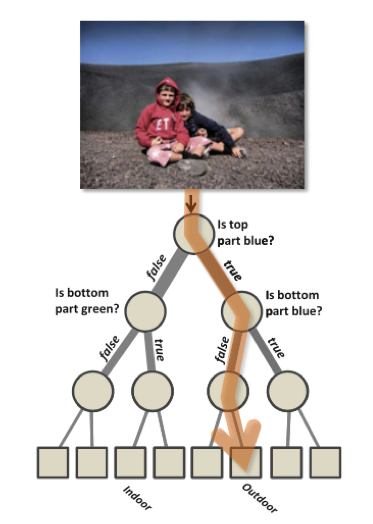
\includegraphics[scale=0.5]{decisiontree.png}
\caption{Diagram of a decision tree for determining whether an image is taken outdoors}
\end{figure}

Our method uses regression forests, which contain regression trees instead of decision trees. Regression trees are the same as decision trees except each leaf node contains a regression model instead of a classification model. Therefore each leaf node would predict a regression value instead of a classification label.

\begin{figure}
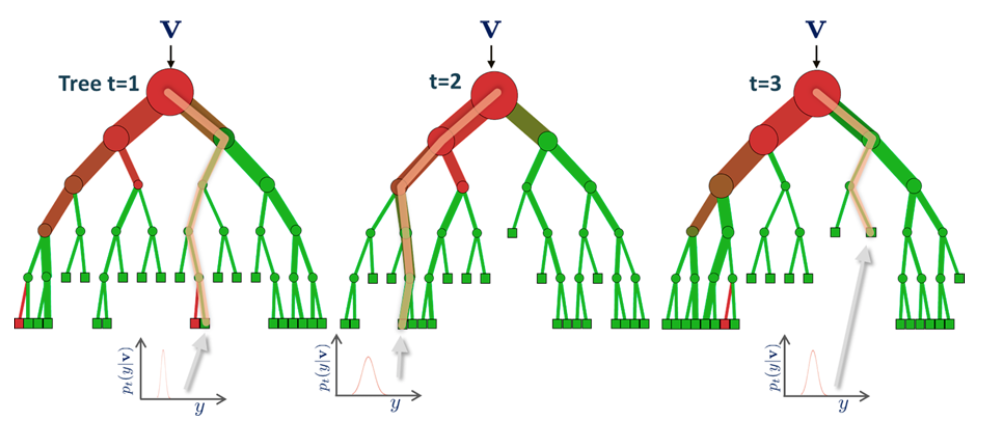
\includegraphics[scale=0.45]{regressionforest.png}
\caption{Diagram of a regression forest consisting of 3 trees and a depth of 5}
\end{figure}

\begin{figure}
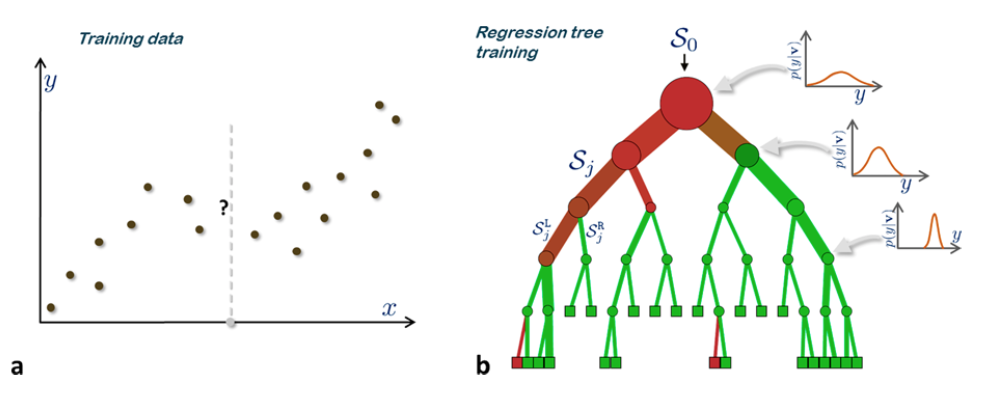
\includegraphics[scale=0.45]{regressiontraining.png}
\caption{Training a regression tree: a) depicts a potential split function, and b) depicts the regression tree}
\end{figure}

A regression forest is produced by aggregating many regression trees. Figure 2 shows a regression forest consisting of only 3 trees, and for each tree a data point can be seen passing through the tree's branches and down to the leaf node, where it is put into a regression model. In the case of this paper, the regression model at the leaf nodes is a Gaussian distribution.
  
A regression forest can be trained by individually training its regression trees. Regression trees are trained by minimizing some loss function at each node. This paper uses information gain, given below:

\begin{equation}
  I(S,\theta) = H(S) - \frac{|S^L|}{|S|} H(S^L) - \frac{|S^R|}{|S|} H(S^R)
\end{equation}
where $S$ is the dataset that reaches that node, $\theta$ denotes the parameters of the function being considered at the split node, $S^L$ is the subset that will go to the left node, and $S^R$ is the subset that will go to the right node, and $H(S)$ is the entropy of a dataset $S$, given below:

\begin{equation}
  H(S) = \frac{1}{2} n \log(2\pi e  |\Sigma|)
\end{equation}

where $\Sigma$ is the covariance matrix of the Gaussian model that is fitted to the dataset at the node. We maximize information gain as the method for choosing a split function, because it will choose the function that will separate the dataset the most. Intuitively, this results in greedily training the tree such that each time the tree branches, we get the most information out of the dataset that ends up at a certain branch.

To train a regression tree, we greedily choose the split functions at each node. At each node, $K$ features are randomly selected, and the feature that maximizes the information gain given above is chosen as the split function for that node. Figure 3 depicts how a selected feature divides the training set, and then Gaussian distributions are fitted to the resulting split nodes. After each regression tree is trained, the set of these trees becomes the regression forest. The introduction of randomness in feature selection is meant to prevent overfitting: each tree is a weak learner, but the aggregation of many randomly trained weak learners should be a strong learner. Training many weak learners in parallel is also computationally much faster than training one strong learner such as a deep regression tree. Once a regression forest is trained, it can make predictions on new data points by running the data point through each of the regression trees until it reaches a leaf node, and combining the outputs of each regression tree. Training a tree terminates either when the maximum tree depth has been reached, or when the information gain is less than some threshold value.

Three hyper-parameters determine the structure of the regression forest: $T$ is the number of trees, $D$ is the maximum tree depth, and $K$ is the number of features being considered at each node.

\section{Method}
\subsection{Regression Forests for Localization of the Heart}
We trained a regression forest to predict the location of the bounding box of the heart given MRI scans of patients with congenital heart disease. Instead of running each entire image through the tree, we run features for each voxel through the tree, and each of those will define a distribution of where the bounding box is. Our method for calculating features for each voxel is described in section 4.2. We can aggregate the distributions from each voxel to get a final distribution for where the bounding box should be. A bounding box is given by a 6-dimensional vector: $(x_1, x_2, y_1, y_2, z_1, z_2)$. $x_1$ and $x_2$ denote the x-values of the two faces of the bounding box that are perpendicular to the $x$-axis, where $x_1$ is the smaller of the two values, and $y_1, y_2, z_1, z_2$ are similarly defined for the other axes.

For each voxel $\mathbf{p}=(p_x, p_y, p_z)$ that we run through the regression forest, we calculate its offset from the bounding box $\mathbf{b}$:
\begin{equation}
  d(\mathbf{p}, \mathbf{b}) = (x_1, x_2, y_1, y_2, z_1, z_2) - (p_x, p_x, p_y, p_y, p_z)
\end{equation}
The Gaussian model fitted at each node is then a 6D Gaussian, representing the voxel's predicted offset from the bounding box. Each of the leaf nodes has a distribution of the voxel's offset from the bounding box, not the bounding box locations themselves.

To produce predictions for the bounding box of a heart given a 3D image, we take each voxel in the image and run it through the regression forest. For each voxel, we can combine the Gaussian distributions resulting from each tree in the forest by sampling the distributions. Then, we add the voxel's location to get the distribution of the predicted absolute location of the bounding box. Then, we combine the distributions from each voxel to form the predicted distribution of the absolute bounding box of the heart.

\subsection{Feature Selection}
As mentioned previously, at each split node, $K$ features are chosen randomly for consideration as the split feature. Each feature is calculated as the mean intensity of voxels in a rectangular box, that is at some offset to the voxel. Therefore, each feature is governed by the following parameters: $\theta$ is the offset to the center of the box, which is a 3D vector, and $\phi$ is the size of the box, which is also a 3D vector. Each dimension of the box must be odd, to ensure that the center of the box is on a lattice point. A feature is calculated with the following equation:

\begin{equation}
  F_{\theta, \phi} = \frac{1}{|B|} \sum_{v \in B} J(v)
\end{equation}
where $B$ is the set of voxels that lie in the box that is described by an offset of $\theta$ and a box size of $\phi$, and $J(v)$ describes the intensity at the voxel $v$. Presence of certain features in the image, such as bright or dark spots, can hint at where the heart is. Therefore, having an especially high or low mean intensity of voxels at a specific offset can contribute a good prediction as to where the heart may be.

To generate a random feature, we sample $\theta$ and $\phi$ from uniform distributions. Each element of $\theta$ is sampled from a uniform distribution from 0 to a fixed fraction of the size of the image in that dimension. Each element of $\phi$ is sampled from a uniform distribution of 1 to $2k+1$ for some $k$. We have not been able to tune parameters much, and currently the parameters are set at $\frac{1}{6}$ of the image size for $\theta$, and $k = 5$ for $\phi$. 

\section{Results}
\subsection{Dataset}
The dataset consists of 3D cardiovascular MRI scans of 10 different patients, which have a variety of congenital heart defects. Manual segmentation was performed on each of the 10 scans, taking around 8 hours each. Image dimension varied across patients, but was 340 x 340 x 140 on average, after resampling the voxel size to 1 x 1 x 1 mm. To evaluate the performance of the proposed method, the regression forest was trained on 9 patients and tested on the remaining patient. Figure 4 shows the ground truth bounding box of a patient's heart as viewed from three different axes.

\begin{figure}
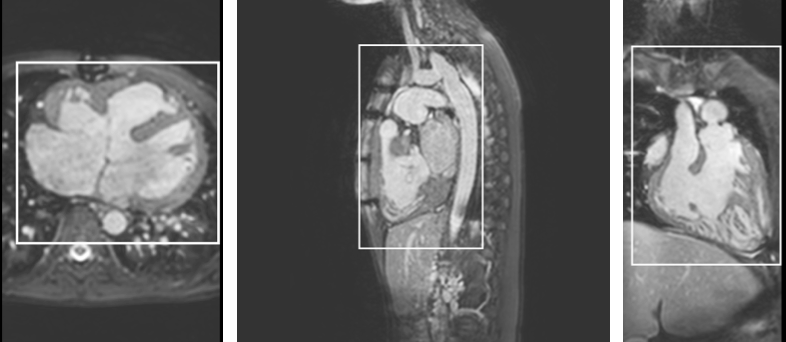
\includegraphics[scale=1.0]{boundingboxes.png}
\caption{Ground truth bounding box of patient 0, as viewed from three different axes}
\end{figure}

\subsection{Localization Error}
As mentioned in section 4.1, to produce a prediction for the bounding box of a heart, each voxel in a 3D image is run through the regression forest, and then the Gaussian distributions at the leaf nodes are combined by sampling the distributions. As described earlier, a bounding box is represented as a 6-dimensional vector, so most likely bounding box is calculated by finding the value with the maximum probability for each element in the vector. We calculate two types of errors: the first is the voxel error, which is the L1 norm of the error between the true bounding box and the calculated most likely bounding box. The second is the percentage error, which is the L1 norm of the same error but each element in the vector is expressed as a percentage of the image size in that dimension.

For each patient in the dataset, we trained the regression forest on the other nine patients and then applied the forest on the remaining patient to find the voxel error and the percentage error. Since there is randomness in the training process, the results are averaged over three runs of the algorithm.

\begin{equation}
  E_1 = \frac{1}{6} \sum_{i=1} ^ {6} |b_i - B_i|
\end{equation}
\begin{equation}
  E_2 = \frac{1}{6} \sum_{i=1} ^ {6} \frac{|b_i - B_i|}{S_{i}}
\end{equation}
where $B$ is the true bounding box, $b$ is the calculated bounding box, and $S_i = (s_1, s_1, s_2, s_2, s_3, s_3)$ where $s_i$ is the size of the image in dimension $i$.

\begin{table}
  \caption{Localization errors [to be filled in later]}
  \label{tab:err}
  \begin{tabular}{p{2cm}p{2cm}p{2cm}}
    \toprule
    Patient Number & Voxel Error (voxels) & Percentage Error (\%) \\
    \midrule
    0 & 0 & 0\\
    1 & 1 & 0\\
    \bottomrule
  \end{tabular}
\end{table}

The above results are obtained by using a regression forest with 10 trees, a maximum tree depth of 8, and 10 randomly selected features at every split node. The image was sampled at a rate of one voxel for every 9x9x9 cube. As shown above [not filled in yet], the percentage errors are relatively small.

[insert a three slice image comparing true bounding box with calculated bounding box]

\subsection{Varying Parameters}
To investigate the effect of varying the regression forest parameters, we decided to vary 4 different parameters and observe the percentage error while testing on patients 2 and 4. We mainly focused on testing with patient 2 and 4, because patient 2 is an example of a more normal-case scenario [help how to reword this] while patient 4 is a baby and therefore an example of a harder case to deal with.
\subsubsection{Number of Trees}

\subsubsection{Maximum Tree Depth}
\subsubsection{Number of Features Considered at Each Split Node}
\subsubsection{Sampling Rate}


\section{Bibliography}
[1] D. Pace, A. Dalca, T. Geva, A. Powell, M. Moghari, P. Golland, Interactive Whole-Heart Segmentation in Congenital Heart Disease

[2] A. Criminisi, J. Shotton (eds.), Decision Forests for Computer Vision and Medical Image Analysis, Advances in Computer Vision and Pattern Recognition




\end{doublespacing}

%If your citations are not being added properly, the solution may be in README
\bibliographystyle{abbrv}
\bibliography{sample_bib}

\end{document}
